\section{Results}
\label{sec:four}

Using the framework and models with their respective parameters as mentioned
above, we obtain the following results.

\begin{figure*}[h]
\centering
\begin{minipage}{.49\textwidth}
  \centering
  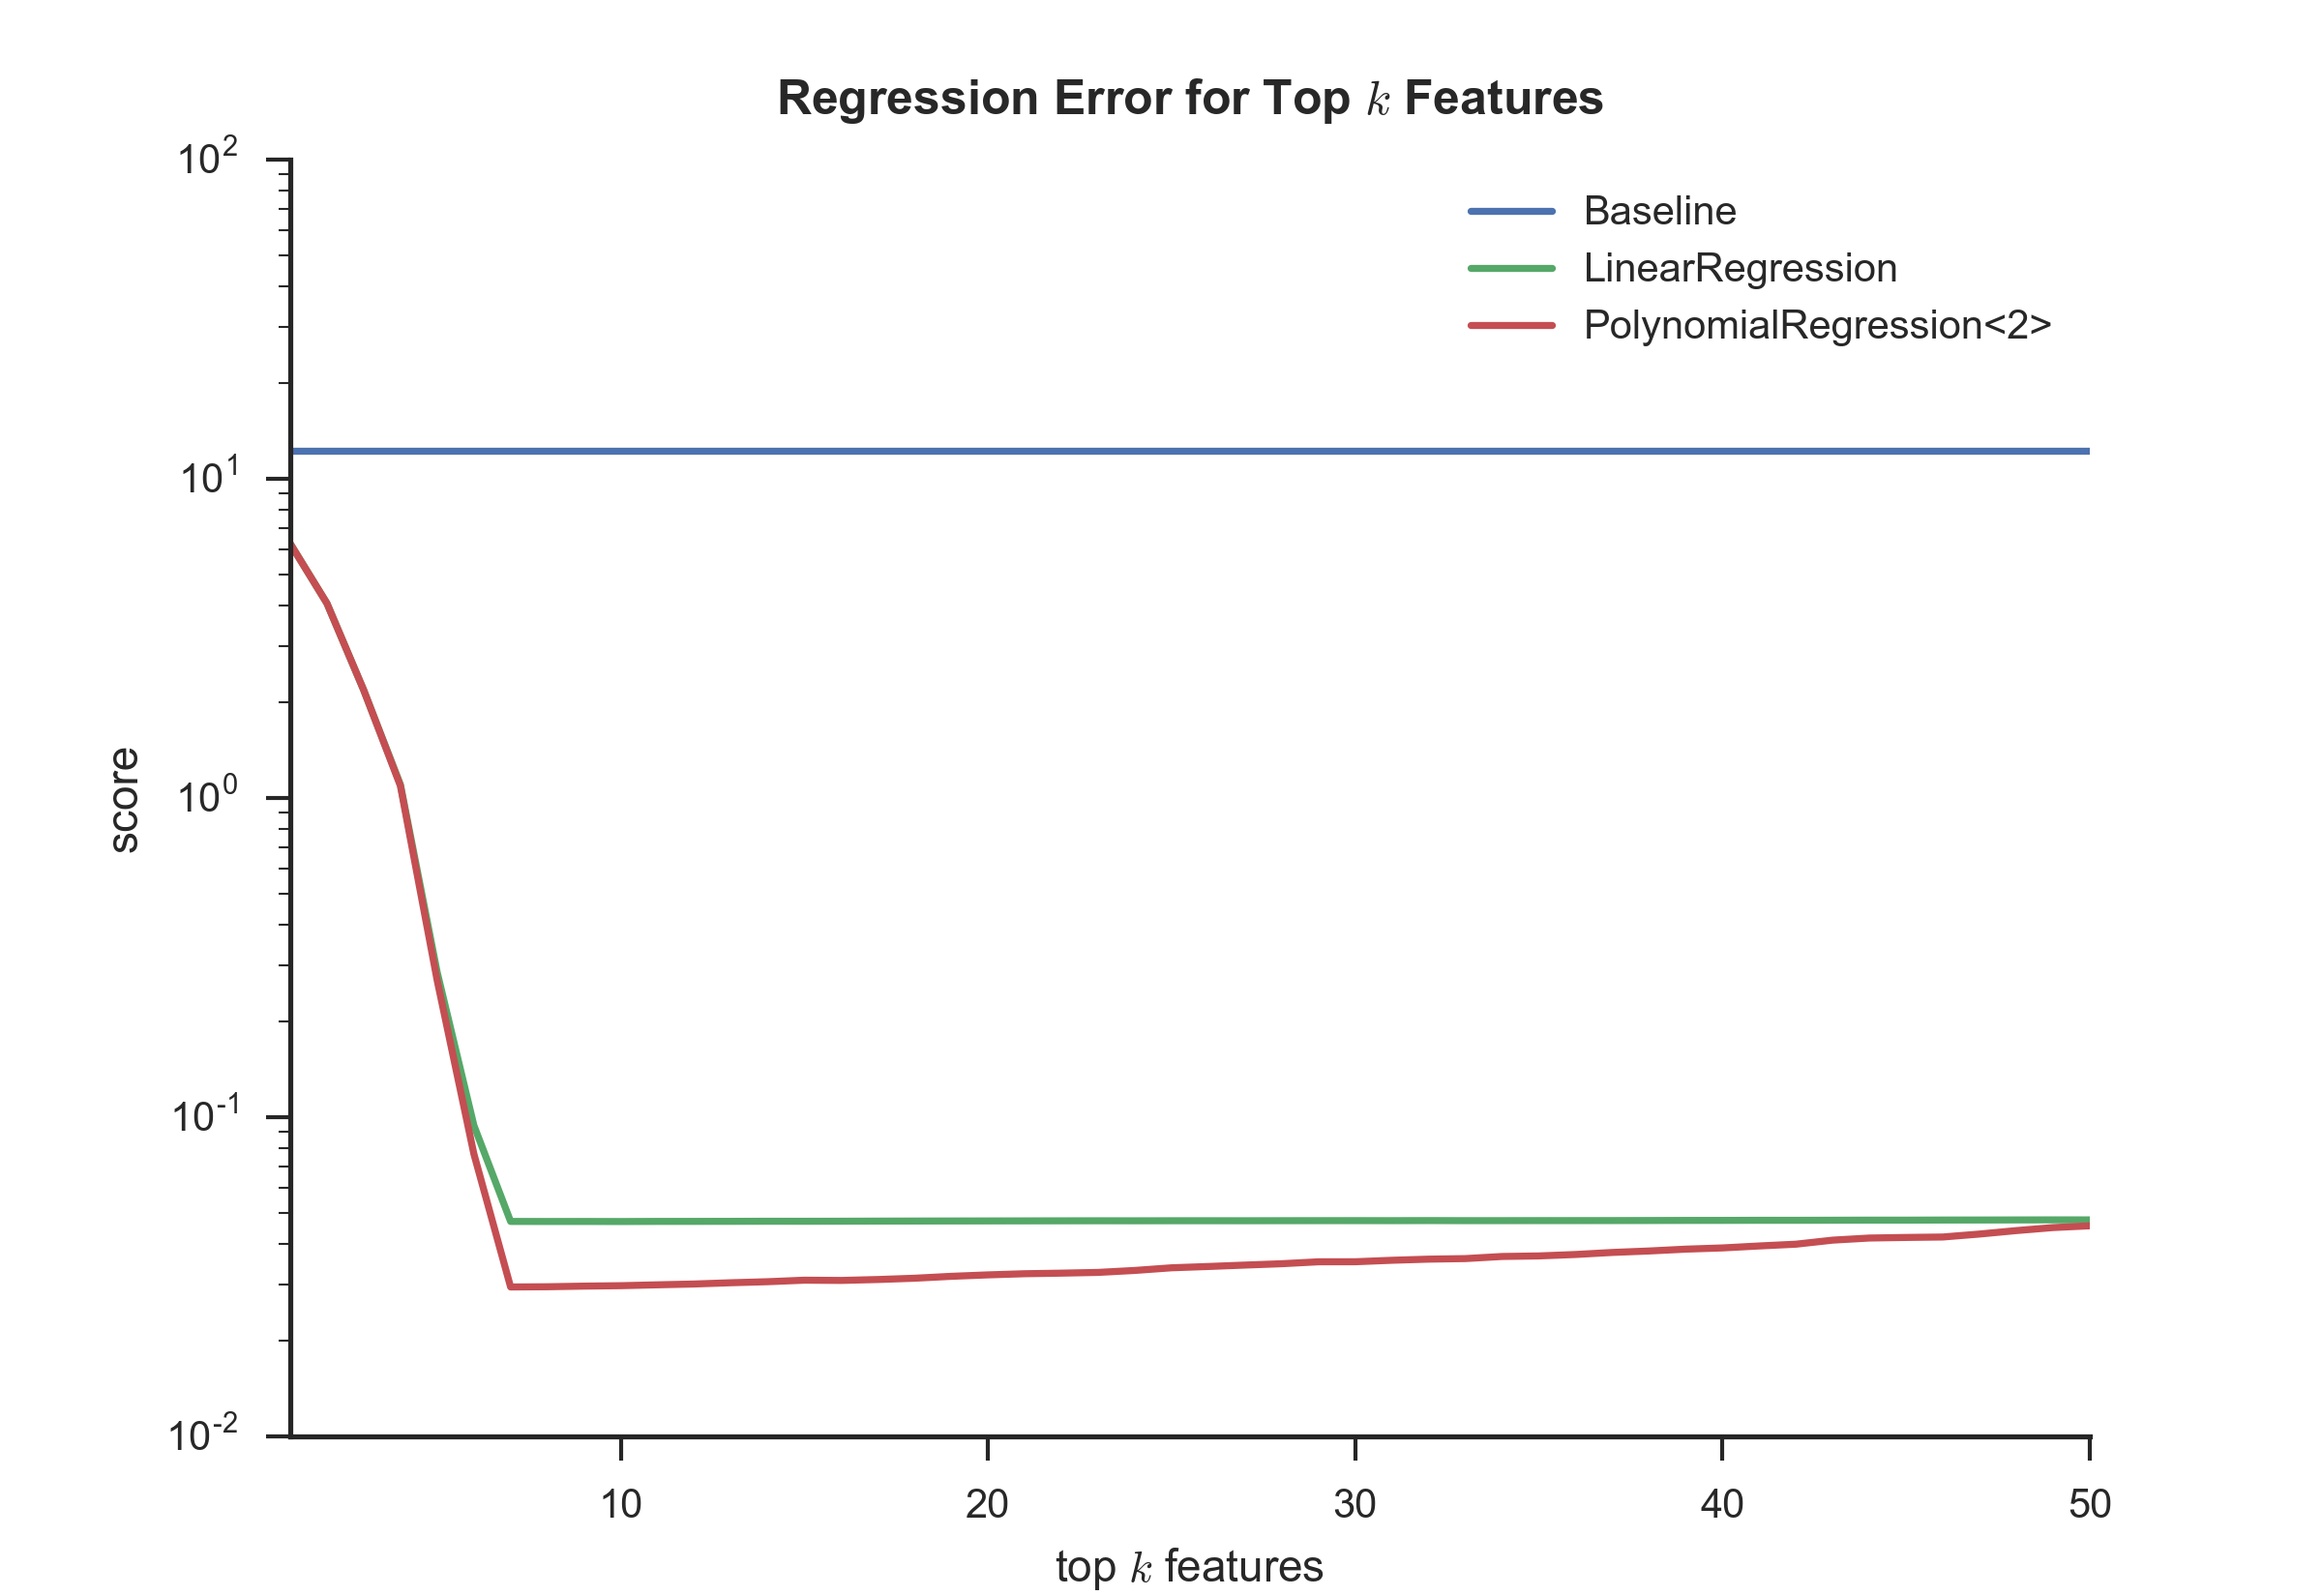
\includegraphics[width=\linewidth]{figures/reg_mse_train.png}
\end{minipage}
\begin{minipage}{.49\textwidth}
  \centering
  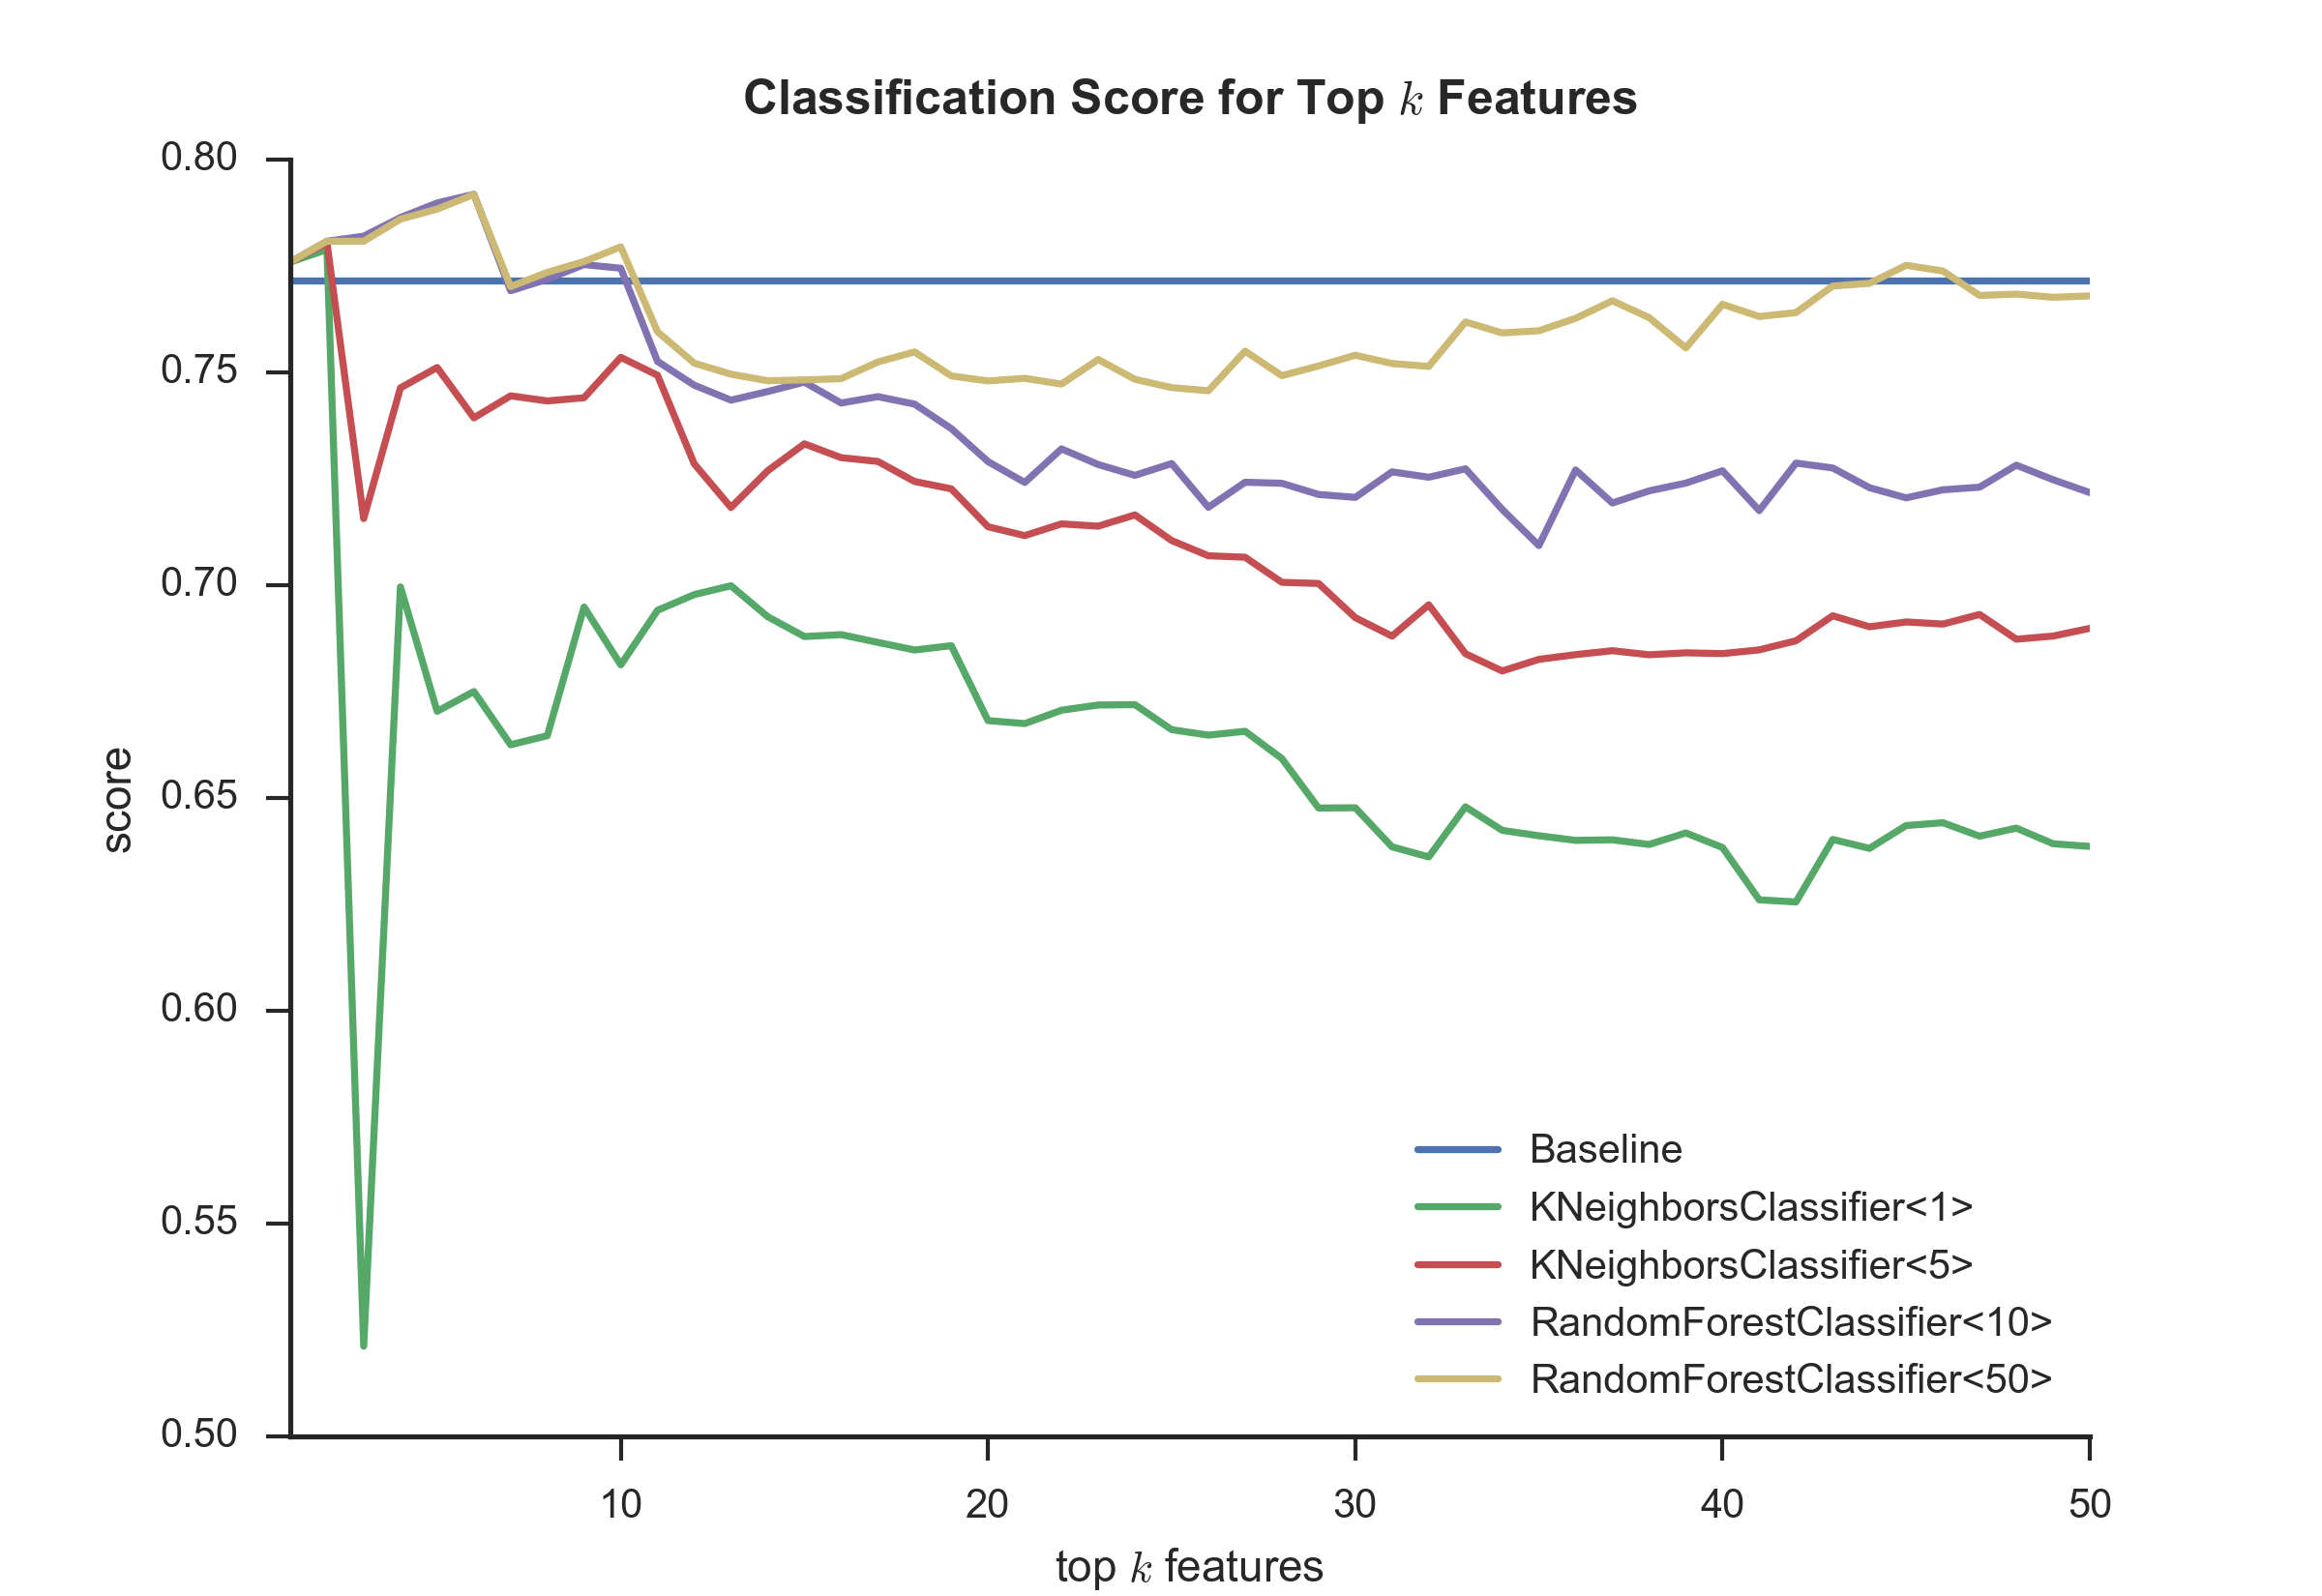
\includegraphics[width=\linewidth]{figures/cls_fscore_train.png}
\end{minipage}
\caption{Performance graphs for regression (left) and classification (right) for
  number of top-$k$ features, evaluated with MSE and \fmeasure, respectively.}
\label{fig:training}
\end{figure*}

\subsection{Regression}

Here, we evaluate three models using cross-validation: baseline (target
average), linear and polynomial regression (of degree two) models for different
subsets of the top-$k$ features.  The MSE yields the scores used to measure the
performance of each model.  The final results are presented in the left-hand
graph of Figure~\ref{fig:training}.

The linear, as well as the polynomial regression model easily outperform the
baseline average.  Polynomial regression produces slightly better scores for
almost all subsets of top-$k$ features than its linear counterpart.  The best
performances is achieved with different subsets for the linear and polynomial
models, top-10 and top-7, respectively.  For these two $k$, we encounter a
minimum for the performance.  With increasing $k$, the performance becomes
worse due to the increasing correlation between the features.

In practice, we choose the polynomial regression model with 7 top-$k$ features
as the final candidate and report only the performance on the test set.  For
demonstration purposes, we additionally consider the baseline and linear
regression model with their respective best top-$k$ values.  The results are
presented in Table~\ref{tab:regperf}.  The polynomial model still outperforms
both models and beats the baseline by a significant margin.

\begin{table}[t]
  \caption{Regression performance comparison of (1) baseline, (2) linear
    regression and (3) polynomial regression of degree two as measured using the
    mean squared error on the test data set.}
  % \centering\small
  % \renewcommand{\tabcolsep}{1pt}
  \newcolumntype{C}{>{\centering\arraybackslash}X}%
  % \newcolumntype{R}{>{\raggedleft\arraybackslash}X}
  \begin{tabularx}{\linewidth}{@{\kern3pt}cCc@{\kern3pt}}
    \toprule
    \bfseries Model & \bfseries Top-$k$ Features & \bfseries MSE \\
    \midrule
    (1) & --- &  12.60835 \\
    (2) &  10 &  0.047144 \\
    (3) &  7  &  0.032311 \\
    \bottomrule
  \end{tabularx}
\label{tab:regperf}
\end{table}

\subsection{Classification}

We apply the same procedure as above for the classification task.  The
right-hand graph in Figure~\ref{fig:training} shows \fmeasure{} scores of the
baseline model (average target), $k$-NN classifiers with $k = 1$ and $k = 5$,
and random forest classifiers with 10 and 50 trees.

Only random forests with a small number of features manage to beat the baseline
model.  Both random forest settings achieve the best result when using top-$k$
subset of 6 features.  The performance worsens with increasing number of $k$
features before slightly improving with even greater numbers of $k$.  The model
with 50 trees performs best overall.

The $k$-NN classifiers barely manage to beat the baseline when using top-$k$
subsets of 1 and 2 features.  Both models achieve the best result with 2
features, with performance decreasing significantly with increasing $k$.  A very
unexpected dip in the performance occurs with $k = 1$ neighbors and a top-$k$
subset of 3 features (and for 2 features in the test data).  We assume that this
phenomenon is due to added noise to the third and second top feature in the
training and testing data sets, respectively, creating an opposite correlation.
This is partially confirmed when comparing the results to the $k$-NN model with
5 neighbors.

Our final model we choose is random forest with 50 trees and using 6 best
selected features. For demonstration purpose, we train all models with the best
settings and run on the test data. The results are presented in the
Table~\ref{tab:clsperf}

Our final model still returns the best result on the data set although by not
much when comparing to the baseline. Other models surpass the baseline by a
small margin as well, except for k-NN with 1 neighbor and 2 features which gives
a very low performance.

\begin{table}[t]
  \caption{Classification performance comparison of (1) baseline, $k$-NN with
    (2) 1 and (3) 5 neighbors, random forest with (4) 10 and (5) 50 decision
    trees as measured using the \fmeasure{} on the test data set.}
  % \centering\small
  % \renewcommand{\tabcolsep}{1pt}
  \newcolumntype{C}{>{\centering\arraybackslash}X}%
  % \newcolumntype{R}{>{\raggedleft\arraybackslash}X}
  \begin{tabularx}{\linewidth}{@{\kern3pt}cCc@{\kern3pt}}
    \toprule
    \bfseries Model & \bfseries Top-$k$ Features & \bfseries \fmeasure{} \\
    \midrule
    (1) & --- & 0.771499 \\
    (2) &   2 & 0.024242 \\
    (3) &   2 & 0.782774 \\
    (4) &   6 & 0.813008 \\
    (5) &   6 & 0.813513 \\
    \bottomrule
  \end{tabularx}
\label{tab:clsperf}
\end{table}

%%% Local Variables:
%%% mode: latex
%%% TeX-master: "../main"
%%% End:
